\documentclass[aspectratio=169,15pt,]{beamer}
\usepackage [utf8] { inputenc }
\usepackage [T1] {fontenc}
\usepackage{carlito}
\usepackage{algorithm}
\usepackage[noend]{algpseudocode}

\title{Solving the optimal path planning of a mobile robot using improved Q-learning - postęp prac}
\institute{WYDZIAŁ ELEKTRONIKI, FOTONIKI I MIKROSYSTEMÓW}
\date{Projekt Specjalnościowy}
\author[Euclid]{Przemysław Jaskuła \texttt{269995@student.pwr.edu.pl}}
%\date{\today}
\pgfdeclareimage[height=\paperheight,width=\paperwidth]{TG}{flower} 
%\titlegraphic{\pgfuseimage{TG}}
\usetheme[vertical,lang=pl,hr=false,pagenumbers,navigation]{NewPwr}

\begin{document}
\begin{frame}[plain]
\titlepage
\end{frame}
\begin{frame}
\tableofcontents
\end{frame}
\section{Przypomnienie}
\begin{frame}
	\sectionpage
\end{frame}
\subsection{Q-learning}
\begin{frame}
	\subsectionpage
\end{frame}
\begin{frame}
	\centering
	\begin{align*}
	&Q(s_t,a_t) \leftarrow (1-\alpha)Q(s,a)+\alpha \left[ r_{t+1} +\gamma \max_{a_{t+1}} Q(s_{t+1},a_{t+1})\right ] \\
	&s_t  \text{: Obecny stan}\\
	&a_t \text{: Akcja podjęta w stanie }s_t\\
	&r_{t+1} \text{: Nagroda po stanie }s_t\\
	&\alpha \text{: Współczynnik nauki}\\
	& \gamma \text{: Współczynnik dyskontowy}
	\end{align*}
\end{frame}
\begin{frame}
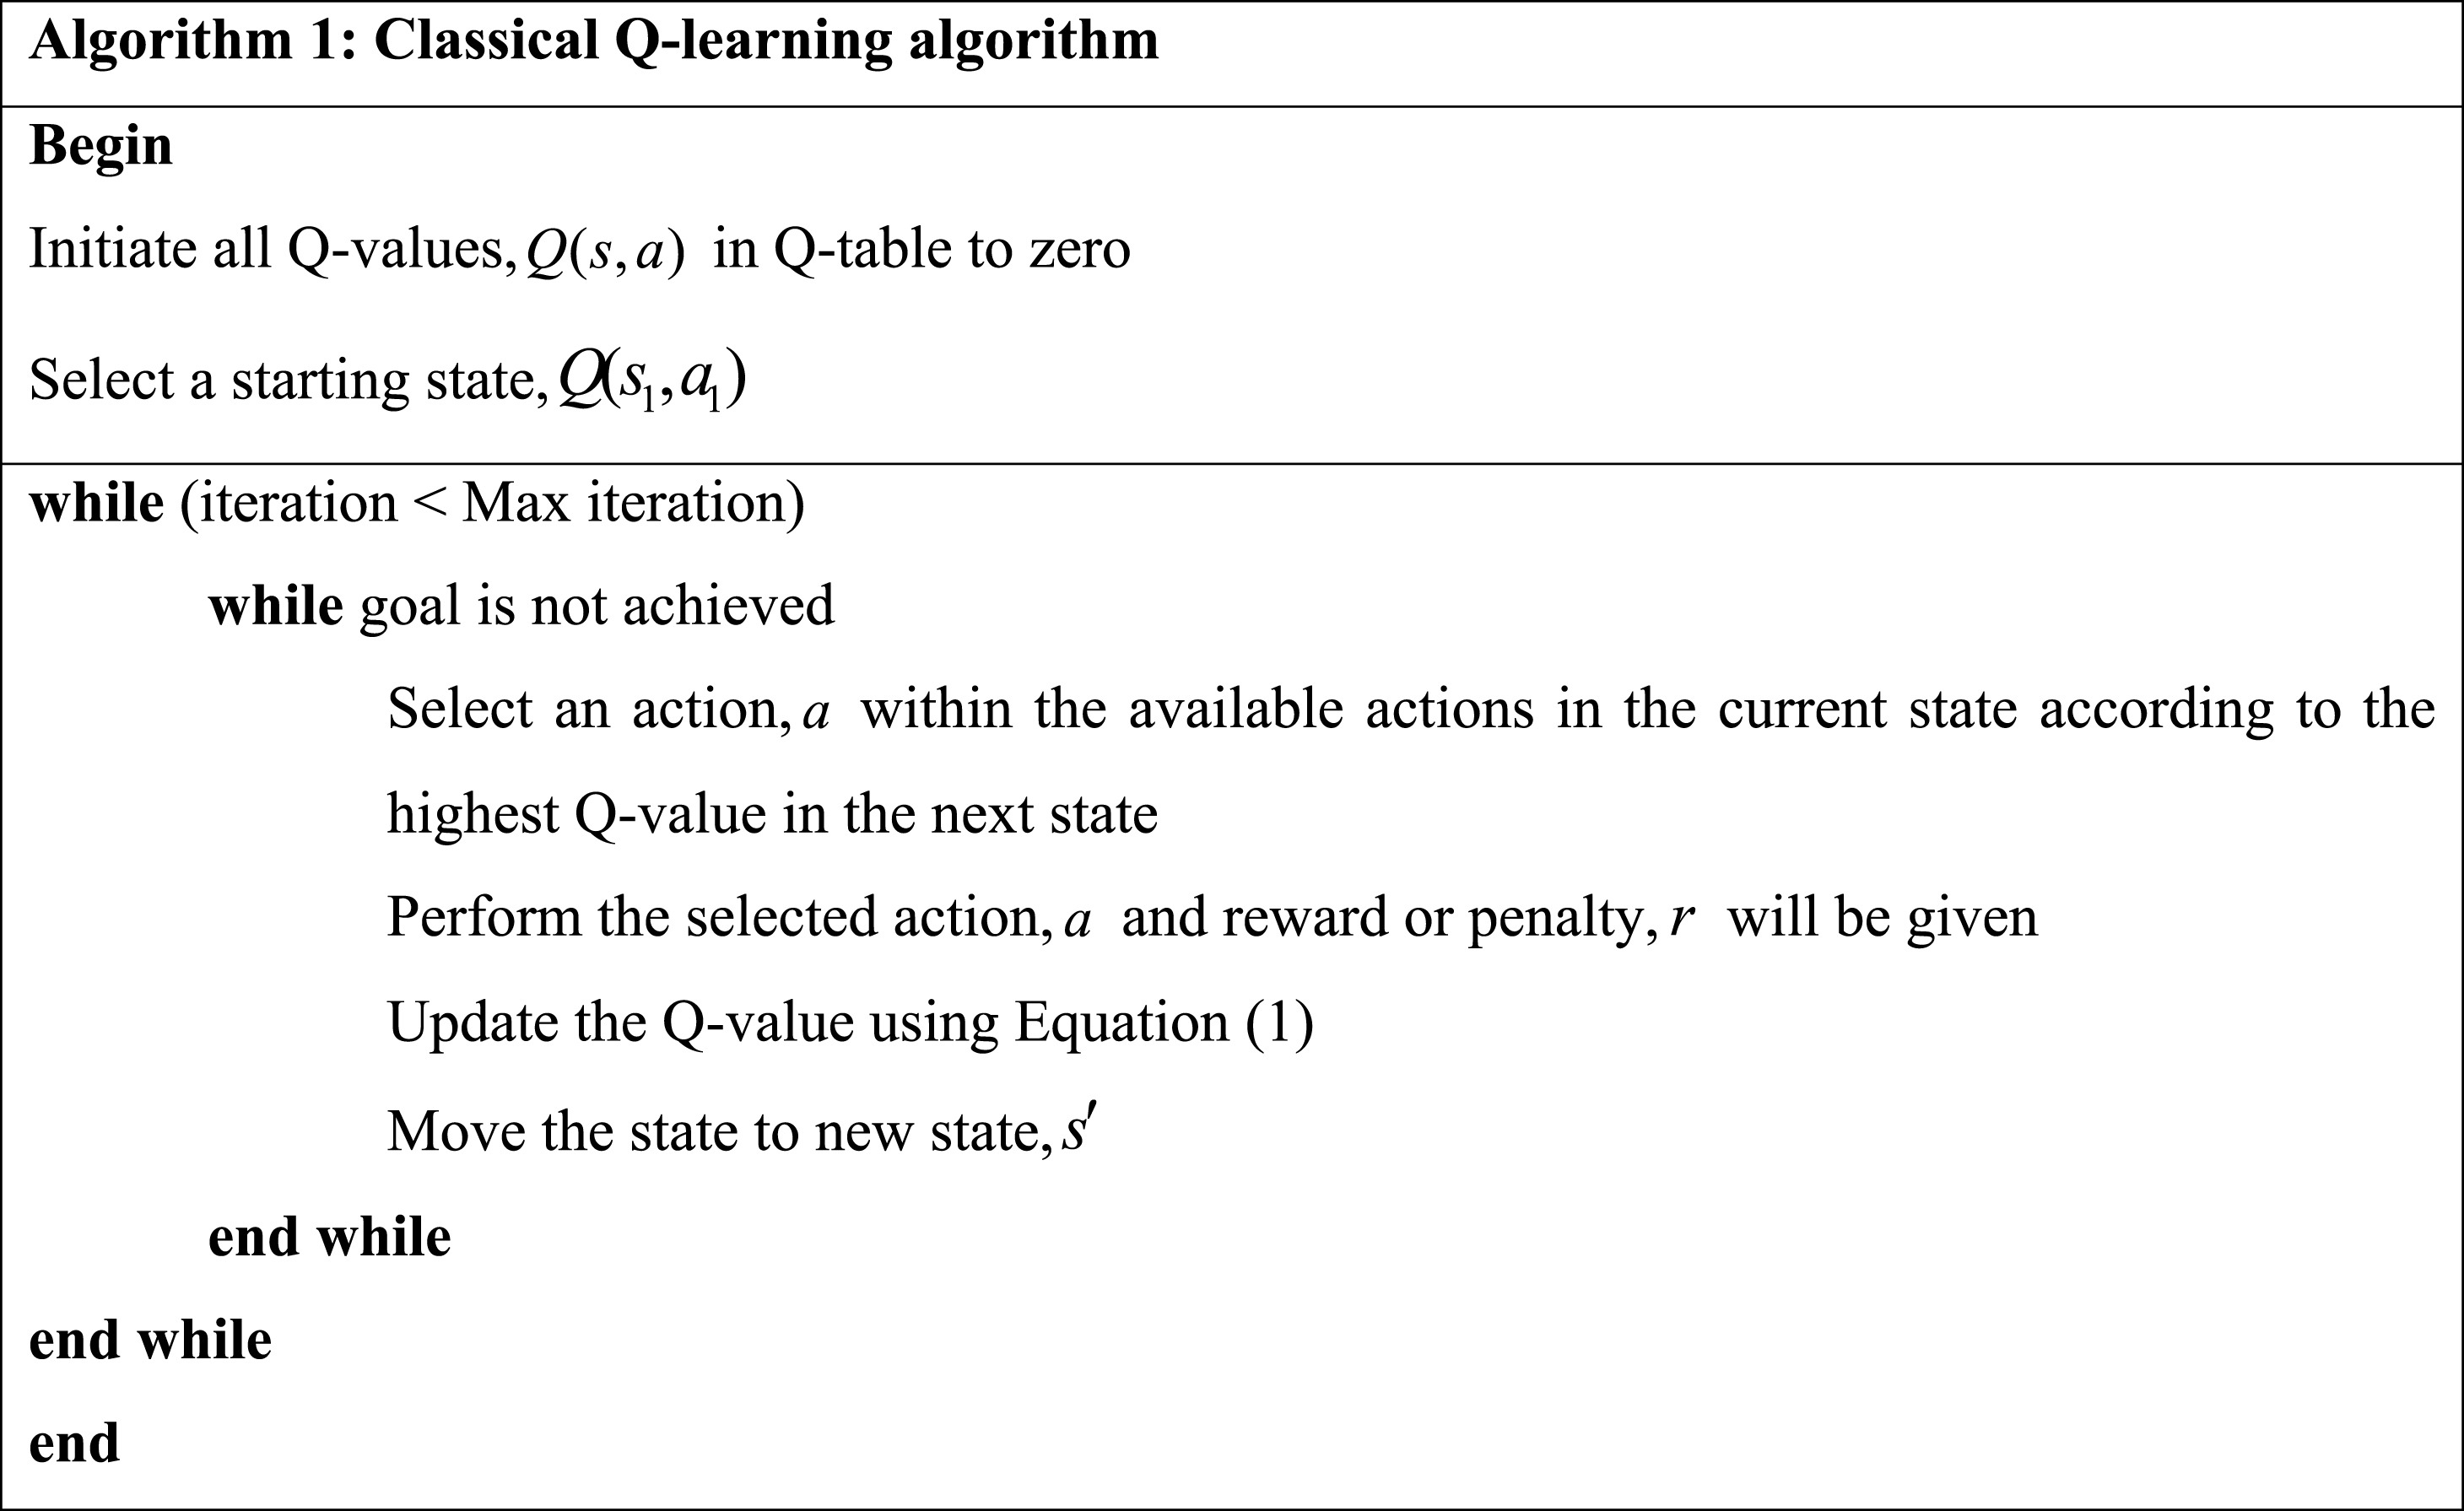
\includegraphics[width =\textwidth]{Obrazy/Pseudo.jpg}
\end{frame}
\subsection{FPA}
\begin{frame}
	\subsectionpage
\end{frame}
\begin{frame}
	\centering
	\begin{align*}
	&x_i^{t+1}=x_i^t +\gamma L (\lambda )(x_i^t - g* ) \\
	&x_i^t  \text{: Pyłek } i \text{ w iteracji } t\\
	&g* \text{: Najlepsze rozwiązanie w obecnej iteracji}\\
	& \gamma \text{: Współczynnik skalowania}\\
	&L(\lambda) \text{: Siła zapylania}
	\end{align*}


\end{frame}

\begin{frame}
	\centering
	\begin{align*}
	&x_i^{t+1}=x_i^t +\epsilon ( x_j^t - x_k^t)\\
	&x_i^t  \text{: Pyłek } i \text{ w iteracji } t\\
	& x_j^t - x_k^t \text{: Pyłki z tego samego gatunku, lecz innych kwiatów}\\
	& \epsilon \text{: Liczba losowa z dystrybucji jednostajnej}
	\end{align*}


\end{frame}

\begin{frame}
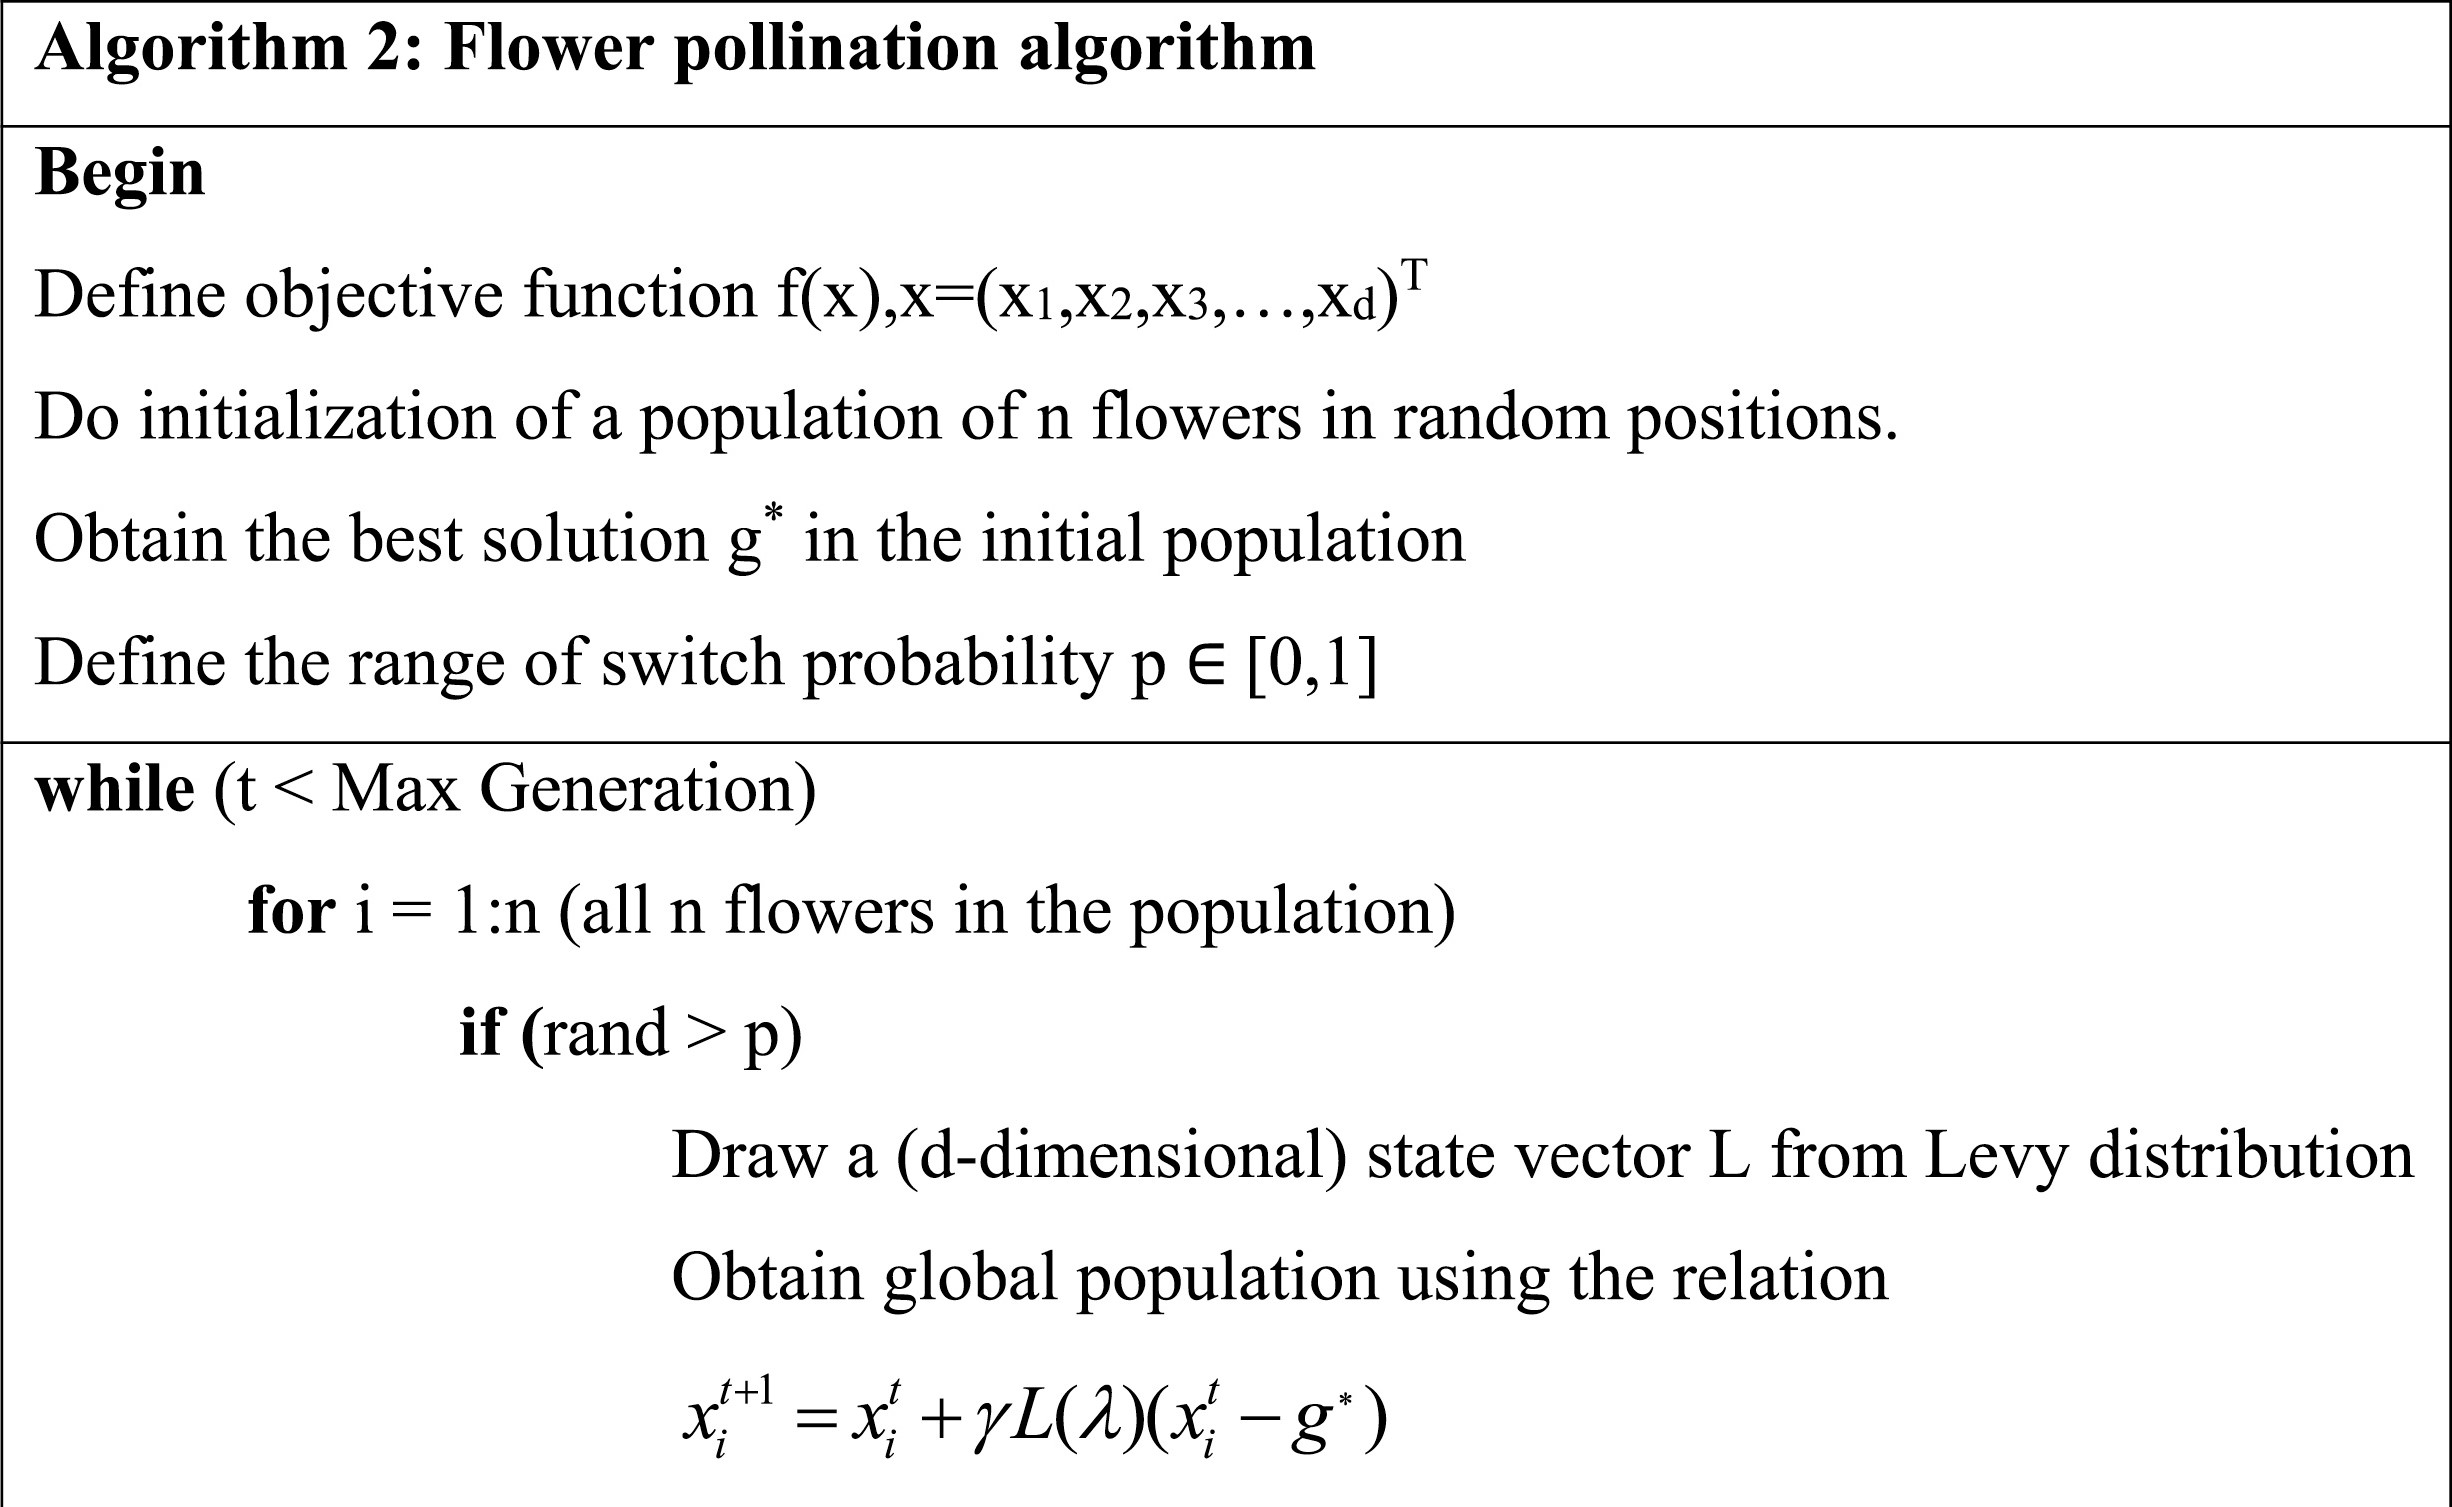
\includegraphics[width =\textwidth,height=\textheight]{Obrazy/Pseudo2.jpg}
\end{frame}
\begin{frame}
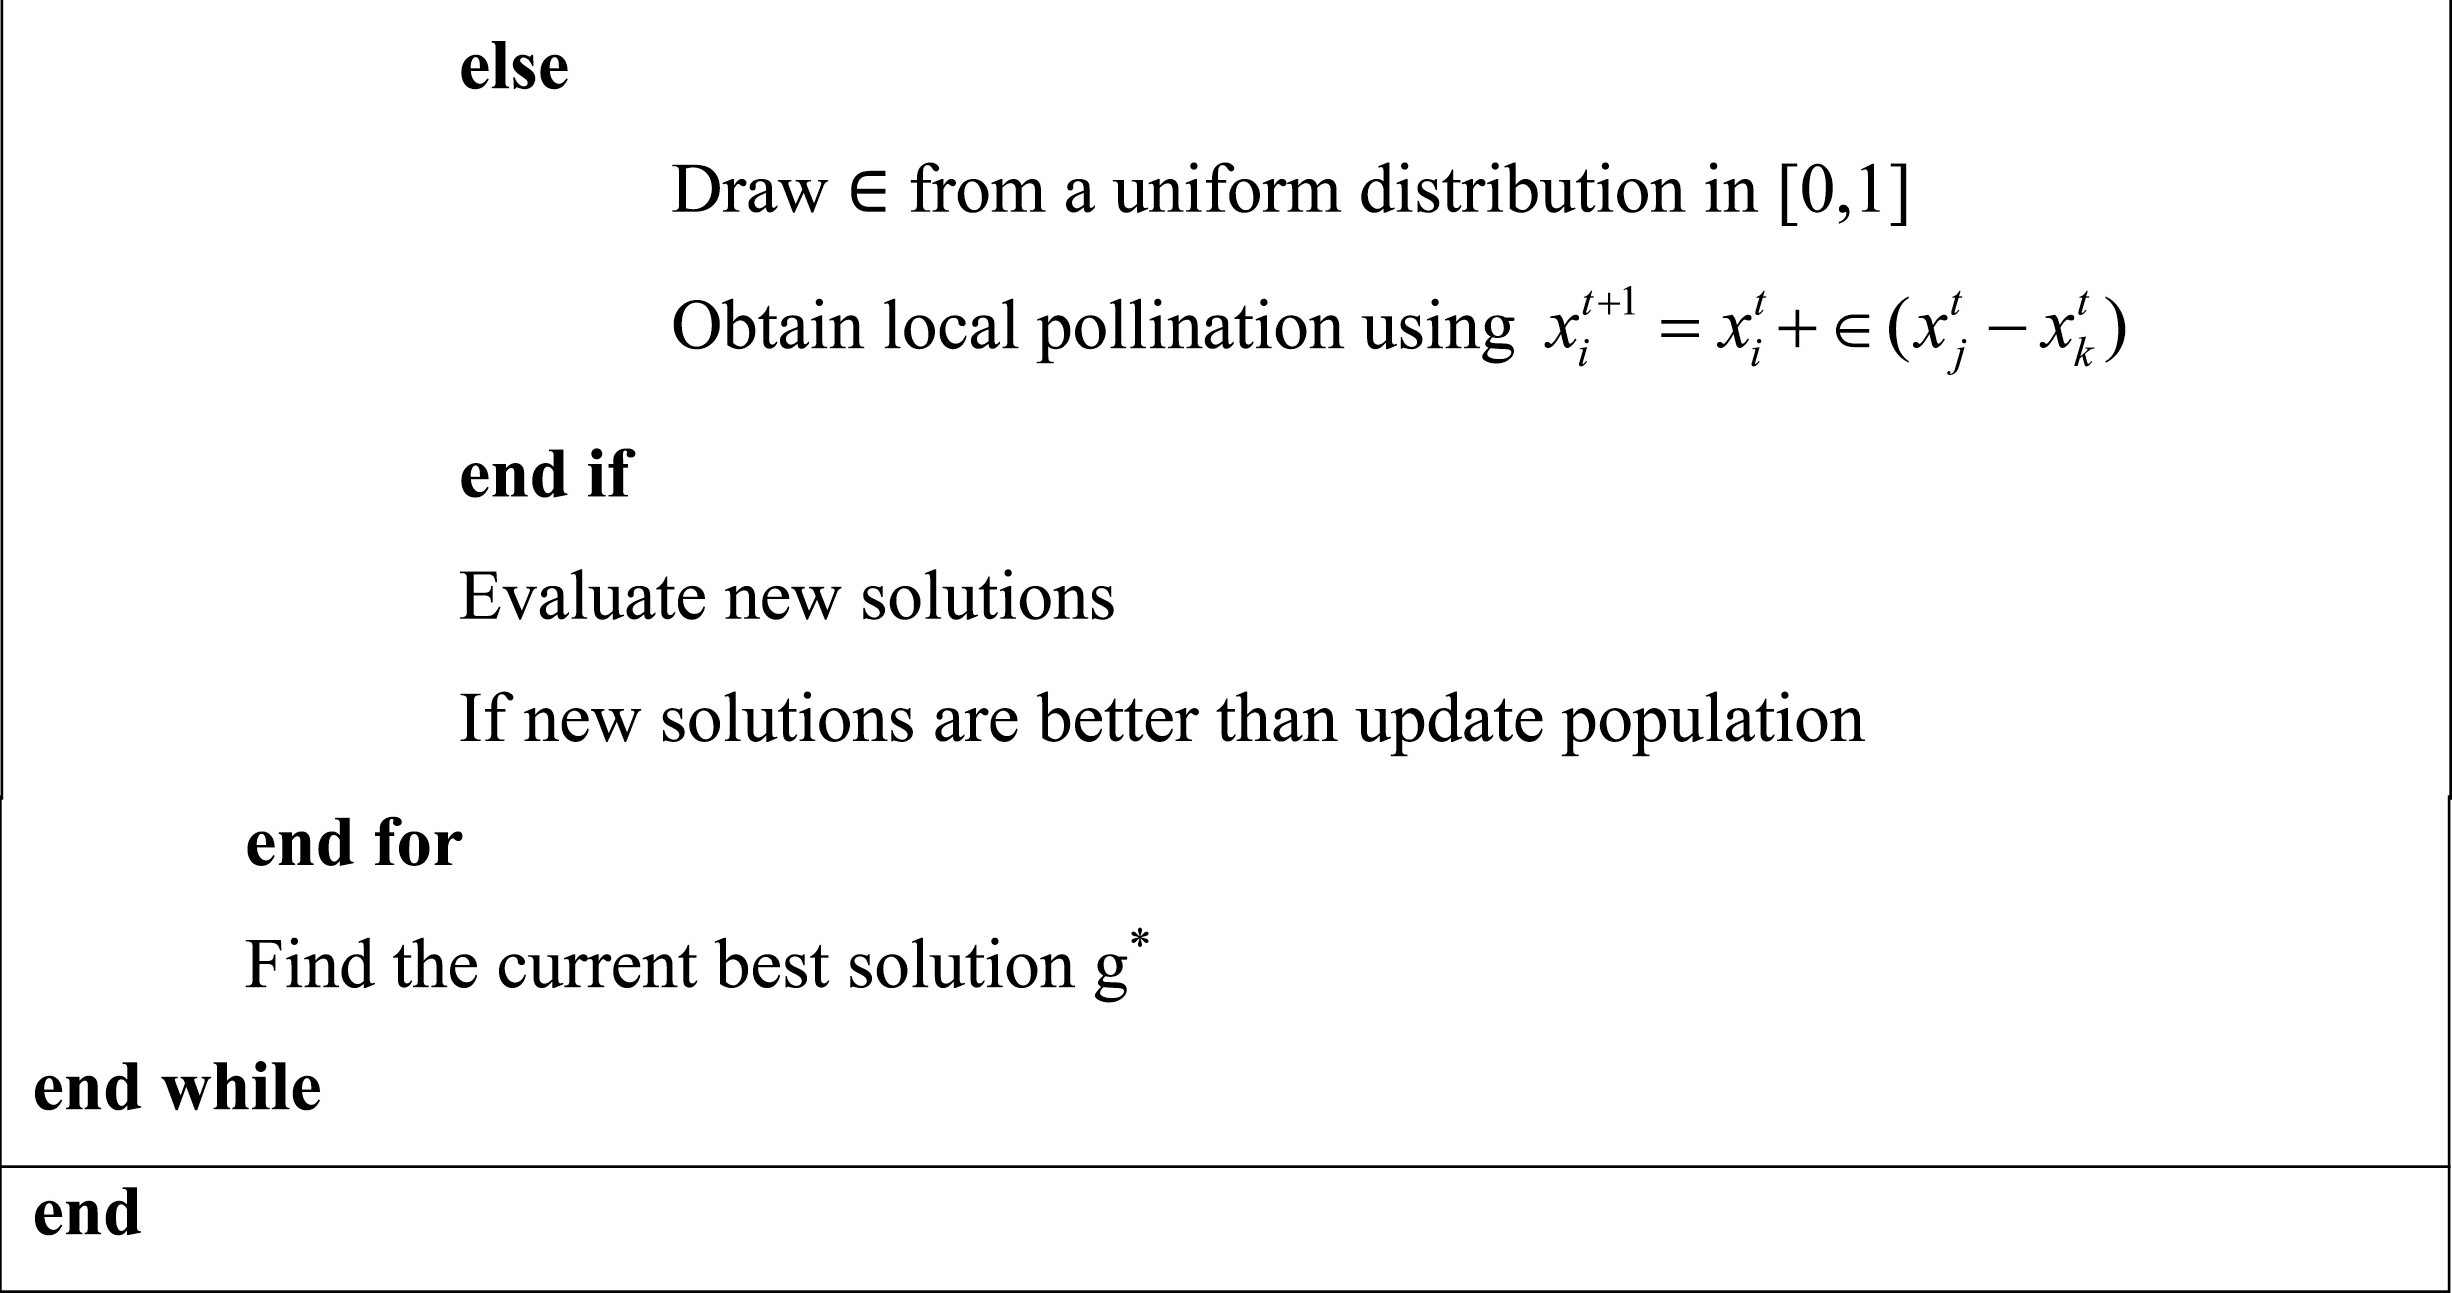
\includegraphics[width =\textwidth,height=\textheight]{Obrazy/Pseudo3.jpg}
\end{frame}
\section{Wyniki}
\begin{frame}
	\sectionpage
\end{frame}
\subsection{Algorytmy w Matlabie}
\begin{frame}
	\subsectionpage
\end{frame}
\begin{frame}
Zdjęcia dróg dla Classic i FPA
\end{frame}

\begin{frame}
Zdjęcia kroków dla Classic i FPA
Classic czas = 1.0034
FPA czas = 0.7780
\end{frame}

\subsection{Wyniki w Ros-Gazebo}
\begin{frame}
	\subsectionpage
\end{frame}

\begin{frame}
Zdjęcia dróg dla Classic i FPA
\end{frame}

\begin{frame}
Zdjęcia kroków dla Classic i FPA
\end{frame}

\begin{frame}
Filmik pokazujący przejazd/ naukę
\end{frame}

\section{Napotkane problemy}
\begin{frame}
	\sectionpage
\end{frame}

\begin{frame}
Blokady w minimach lokalnych( taniec w miejscu)

Powrót do miejsca po przeszkodzie

Czas obliczeń

\end{frame}

\section{Następne kroki}
\begin{frame}
	\sectionpage
\end{frame}

\begin{frame}
Dunno yet

Zaimplementowanie mapy losowej?
\end{frame}

\section{Q \& A}
\begin{frame}
	\sectionpage

\end{frame}

\begin{frame}
\begin{center}
	\Huge{Dziękuję za uwagę}

\end{center}

\end{frame}

\end{document}


